\documentclass[11pt]{article} 
% ~~~~~~~~~~~~~~~~~~~~~~~~~~~~~~~~~~~~~~~~~~~~~~~~~~~~~ %
\input{./Scripts/packages}	
\input{./Scripts/ridefinitions}
\input{./Scripts/figuresgraphicalsettings}
\input{./Scripts/tablesgraphicalsettings}
\input{./Scripts/newcommands}
% Definition of blocks:
\tikzset{%
  block/.style    = {draw, thick, rectangle, minimum height = 3em,
    minimum width = 3em},
  sum/.style      = {draw, circle, node distance = 2cm}, % Adder
  input/.style    = {coordinate}, % Input
  output/.style   = {coordinate} % Output
}
% Defining string as labels of certain blocks.
\newcommand{\suma}{\Large$+$}
\newcommand{\inte}{$\displaystyle \int$}
\newcommand{\derv}{\huge$\frac{d}{dt}$}
% ~~~~~~~~~~~~~~~~~~~~~~~~~~~~~~~~~~~~~~~~~~~~~~~~~~~~~ %

\title{\Huge ELEC-E8101 Group project: \\ Lab A report \\ Group 11}
\date{\today}
\author{HOUILLE Florent, MONTE SASTRE Enrique, SOULARD Yoann, WANG Tong}


\begin{document}
\maketitle

%/////////////////////////////////////////////////////////////%
%/////////////////////////TASK 5.1/////////////////////////%
%/////////////////////////////////////////////////////////////%
\subsection*{Reporting of Task 5.1}

%/////5.1.1/////%


\end{document}

%	INLINE EQUATION FORMAT
% This is an example sentence with this formula : $x=50$

%	BOLD TEXT
%\textbf{Type text here}

%	FRACTION
%\frac{Numerator}{Denominator}

%	 MATRIX with brackets like this : [ ]
%\begin{equation*}
%x=
%	\begin{bmatrix}
%	x_11 x_12\\
%	x_21 x_22\\
%	x_31 x_32\\
%
%	\end{bmatrix}
%\end{equation*}

%	SYSTEM OF EQUATIONS
%\begin{align*}
%\begin{cases}
% equation1 left part = equation1 right part\\
% equation2 left part = equation2 right part\\
%\end{cases}
%\end{align*}

%	1 FIGURE centered just after the text, with a description and a number
%\begin{figure}[H]
%  \includegraphics[width=\linewidth]{LabFolder/ImageName.png}
%  \caption{Description of figure}
%  \label{fig:fig1}
%\end{figure}


%	4 FIGURES displayed 2 by 2 , with a global description
%\begin{figure}[H]
%  \includegraphics[width=\linewidth/2]{LabA/Task45_xw.pdf}
%  \includegraphics[width=\linewidth/2]{LabA/Task45_Thetaw.pdf}
%  \includegraphics[width=\linewidth/2]{LabA/Task45_vw.pdf}
%  \includegraphics[width=\linewidth/2]{LabA/Task45_d.pdf}
%  \caption{Simulation results}
%  \label{fig:fig4}
%\end{figure}

%	4 FIGURES displayed 2 by 2 , with a description for each
%\begin{figure}[H]
%\begin{subfigure}[b]{0.5\linewidth}
%  \includegraphics[width=\linewidth]{LabA/Task48_vmDiscXTraMass0kg500g.pdf}
%  \caption{description 1}
%\end{subfigure}
%\begin{subfigure}[b]{0.5\linewidth}
%  \includegraphics[width=\linewidth]{LabA/Task48_vmDiscXTraMass1kg.pdf}
%    \caption{description 2}
%\end{subfigure}
%\begin{subfigure}[b]{0.5\linewidth}
%  \includegraphics[width=\linewidth]{LabA/Task48_vmDiscXTraMass3kg.pdf}
%    \caption{description 3}
%\end{subfigure}
%\begin{subfigure}[b]{0.5\linewidth}
%  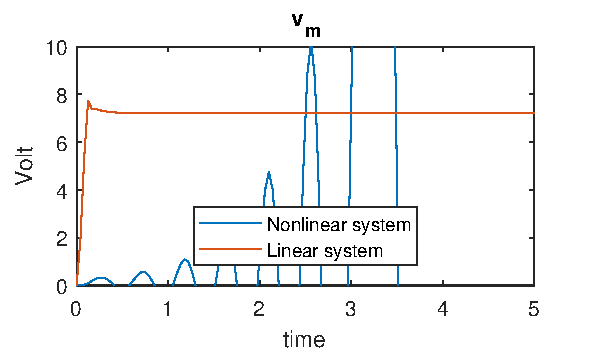
\includegraphics[width=\linewidth]{LabA/Task48_vmDiscXTraMass25kg.pdf}
%    \caption{description 4}
%\end{subfigure}
%  \caption{General description}
%  \label{fig:fig7}
%\end{figure}
